\section{Parabolic variational inequality}
\subsection{}
\begin{frame}
\frametitle{ Parabolic model problem with linear complementarity constraints}
\begin{equation*}
\dps \left\lbrace\begin{array}{llccc} 
\dps \textcolor{red}{\partial_t u_1} -\mu_1 \Delta u_1-\lambda =
f_1 \qquad \hspace{5.75 cm}\mbox{in} \ \quad \Omega \times \left]0,T\right[, \\ 
\dps \dps \textcolor{red}{\partial_t u_2} -\mu_2 \Delta u_2+\lambda =
f_2 \qquad \hspace{5.75 cm} \mbox{in} \ \quad \Omega \times \left]0,T\right[,\\ 
\textcolor{electricpurple}{u_1-u_2} \geq 0, \quad \textcolor{carmine}{\lambda} \geq 0, \quad \dps \textcolor{carmine}{\lambda} (\textcolor{electricpurple}{u_1-u_2}) =0 \hspace{3.8 cm}\mbox{in} \quad \
\Omega \times \left]0,T\right[,\\ 
\dps u_1=g \qquad \hspace{8.3 cm} \mbox{on} \hspace{0.35 cm} \partial \Omega \times \left]0,T\right[,\\ 
\dps
u_2=0 \qquad \hspace{8.32 cm} \mbox{on} \hspace{0.32 cm} \partial \Omega \times \left]0,T\right[,\\
u_1(\bx,0) = u_1^0(\bx), \ u_2(\bx,0) = u_2^0(\bx), \ u_1^0(\bx)-u_2^0(\bx) \geq 0 \hspace{1.1 cm} \mbox{in}  \hspace{0.44 cm} \Omega.
\end{array}
\right.
\end{equation*}
\invisible<1>{
\textcolor{cadmiumgreen}{\textbf{Two possibilities to characterize the weak solution}}\\
\vspace{0.2 cm}
Recall $\Lambda=\left\{\chi\in L^2(\Omega), \: \textcolor{carmine}{\chi \geq 0} \: \mbox{a.e.} \ \mbox{in} \hspace{0.1 cm} \Omega\right\}$
\begin{itemize}
\item Saddle point formulation $(u_1,u_2,\lambda) \in L^2(0,T;H_g^1(\Omega)) \times L^2(0,T;H_0^1(\Omega)) \times L^2(0,T; \Lambda)$
\item Parabolic variational inequality: $\bu \in \Kgt$
\end{itemize}
\beeqn
\Kgt \egaldef \left\{ \bv \in L^2(0,T;H_g^1(\Omega)) \times L^2(0,T;H_0^1(\Omega)), \ \bv(t) \in \Kg \quad \mbox{a.e in} \  ]0,T[\right\}
\eeqn
\invisible<2>{
}}
\end{frame}
%
\begin{frame}
\frametitle{Discrete complementarity problems}
\textcolor{red}{\textbf{$n \geq 1$,} \ \textbf{$p \geq 1$:}} 
\invisible<1>{
\begin{equation*}
\begin{split}
&\bbE^n \Xh^n = \bF^n,\\
&\textcolor{electricpurple}{\X_{1h}^n \hspace{-0.05 cm}+\hspace{-0.05 cm} g {\bf 1} \hspace{-0.05 cm} - \hspace{-0.05 cm} \X_{2h}^n} \geq 0 \   \textcolor{carmine}{\X_{3h}^n} \geq 0 \ \left( \textcolor{electricpurple}{\X_{1h}^n \hspace{-0.05 cm}+\hspace{-0.05 cm} g {\bf 1} \hspace{-0.05 cm}-\hspace{-0.05 cm} \X_{2h}^n} \right) \hspace{-0.05 cm} \cdot \hspace{-0.05 cm} \textcolor{carmine}{\X_{3h}^n} = 0.
\end{split}
\quad 
\bbE^n \hspace{-0.05 cm}
\egaldef \hspace{-0.1 cm}
\left[\begin{array}{ccr}
\hspace{-0.1 cm} \mu_1 \bbS \hspace{-0.1 cm}+\hspace{-0.1 cm} \textcolor{red}{\frac{1}{\Delta t_n} \mathbb{M}} & \mathbf{0} & -\mathbb{D} \\
\mathbf{0} &\mu_2 \bbS \hspace{-0.1 cm}+\hspace{-0.1 cm} \textcolor{red}{\frac{1}{\Delta t_n}} \mathbb{M} & + \mathbb{D}
\end{array}
\hspace{-0.05 cm} \right]
\end{equation*}
% \textcolor{red}{\textbf{$p \geq 2$: Lagrange basis:}}
% \invisible<2>{
% \beeqn
% \begin{split}
% &\widetilde{\bbE}_p^n \Xh^n = \bF^n\\
% &\textcolor{electricpurple}{\X_{1h}^n \hspace{-0.05 cm}+\hspace{-0.05 cm} g {\bf 1} \hspace{-0.05 cm} - \hspace{-0.05 cm} \X_{2h}^n} \geq 0 \   \textcolor{carmine}{\widehat{\mathbb{M}} \X_{3h}^n} \geq 0 \ \left( \textcolor{electricpurple}{\X_{1h}^n \hspace{-0.05 cm}+\hspace{-0.05 cm} g {\bf 1} \hspace{-0.05 cm}-\hspace{-0.05 cm} \X_{2h}^n} \right) \hspace{-0.05 cm} \cdot \hspace{-0.05 cm} \textcolor{carmine}{\widehat{\mathbb{M}} \X_{3h}^n} = 0.
% \end{split}
% \hspace{0.15 cm}
% \widetilde{\bbE}_p^n
% \egaldef \hspace{-0.15 cm}
% \footnotesize{\left[\begin{array}{ccr}
% \hspace{-0.15 cm} \mu_1 \bbS \hspace{-0.05 cm}+\hspace{-0.05 cm} \frac{1}{\Dt_n} \overset{\circ}{\mathbb{M}} & \mathbf{0} & -\widehat{\mathbb{M}} \\
% \hspace{-0.05 cm} \mathbf{0} &\mu_2 \bbS \hspace{-0.05 cm} + \hspace{-0.05 cm} \frac{1}{\Dt_n} \overset{\circ}{\mathbb{M}} & + \widehat{\mathbb{M}}
% \end{array}
% \hspace{-0.15 cm}\right]}
% \eeqn


%%% DUAL BASIS
% \textcolor{red}{\textbf{$p \geq 2$: Dual basis:}}
% \beeqn
% \begin{split}
% & \bbE_{p}^n \Xhn = \bF^n,\\
% & \textcolor{electricpurple}{\X_{1h}^n \hspace{-0.05 cm} + \hspace{-0.05 cm} g {\bf 1} \hspace{-0.05 cm} - \hspace{-0.05 cm} \X_{2h}^n} \geq 0 \ \textcolor{carmine}{\X_{3h}^n} \geq 0 \ \left(\textcolor{electricpurple}{\X_{1h}^n \hspace{-0.05 cm} + \hspace{-0.05 cm} g {\bf 1} \hspace{-0.05 cm} - \hspace{-0.05 cm}\X_{2h}^n}\right) \cdot \textcolor{carmine}{\X_{3h}^n} = 0. 
% \end{split}
% \quad
% \bbE_{p}^n
% \egaldef
% \footnotesize{\left[\begin{array}{ccr}
% \mu_1 \bbS + \frac{1}{\Dt_n} \overset{\circ}{\mathbb{M}} & \mathbf{0} & - \mathbb{I}_{\mathrm{d}}\\
% \mathbf{0} &\mu_2 \bbS + \frac{1}{\Dt_n} \overset{\circ}{\mathbb{M}} & + \mathbb{I}_{\mathrm{d}}
% \end{array}
% \right]}
% \eeqn
\vspace{0.3 cm}
\invisible<2>{
\textcolor{midnightblue}{\textbf{Employing a C-function our problem reads}}
\begin{equation*}
\left\lbrace\begin{array}{llccc}
\bbE^n \X_{h}^n &= \bF^n,\\
\CFun(\X_{h}^n)&=\mathbf{0}.
\end{array}
\right.
\end{equation*}
\vspace{0.3 cm}
\invisible<3>{
\textcolor{midnightblue}{\textbf{Inexact semismooth Newton method:}}
\begin{equation*}
\mathbb{A}^{n,\kk-1} \Xh^{n,\kk,\ii} = \bB^{n,\kk-1} - \bR_h^{n,\kk,\ii}
\end{equation*}
\invisible<4>{
}}}}

\end{frame}
%
\begin{frame}[noframenumbering]
\centering
\Huge{\textcolor{carmine}{A posteriori error estimates}}
\end{frame}

% SLIDE APOS PARABOLIQUE
% \begin{frame}
% \frametitle{A posteriori analysis}
% \textcolor{red}{\textbf{Methodology of equilibrated flux reconstructions:}}
% \newline
% \textcolor{midnightblue}{\textbf{Decomposition of the total flux:}}
% \begin{equation*}
% \sigialfhnki \egaldef \underbrace{\sigialfhdiscnki}_{\in \HdivOmeg} + \underbrace{\sigialfhalgnki}_{\in \HdivOmeg, \ \mbox{\scriptsize{multilevel reconstruction}}} 
% \end{equation*}
% \textcolor{midnightblue}{\textbf{Equilibration property:}}
% \begin{equation*}
% \left(\nab \cdot \sigialfhdiscnki, q_h \right)_K = \left(f_{\ialf} -(-1)^{\ialf} \lambhnki - \rialfhnki - \partial_t \uialfhtaunki,q_h \right)_K \forall q_h \in \Pp(K)
% \end{equation*}
% \begin{equation*}
% \nab \cdot \sigialfhalgnki = \rialfhnki
% \end{equation*}
% \textcolor{midnightblue}{\textbf{Two a posteriori error estimates:}}
% \newline
% 1) At convergence for \textcolor{red}{$\bf \Pone$} finite elements $\uhtau \in \Kgt$: three estimators
% \newline
% 2) Inside the semismooth iterations $\kk \geq 1$ and $\ii \geq 0$ for \textcolor{red}{$\bf \mathbb{P}_p$} finite elements: many estimators 
% \end{frame}
%
\begin{frame}
\frametitle{A posteriori analysis}
\textcolor{cadmiumgreen}{\textbf{We employ the methodology of equilibrated flux reconstructions}}
\vspace{0.4 cm}
\begin{theorem}[Guaranteed upper bound]
\beeqn
\textcolor{red}{\forall p \geq 1}, \ \forall \kk \geq 0, \ \forall \ii \geq 0, \quad \tnorm{\bu-\uhtau^{\kk,\ii}}_{L^2(0,T;\HunzeroOmega)}  \leq \eta^{\kk,\ii}
\eeqn
\end{theorem}
\vspace{0.4 cm}
\begin{corollary}[Distinction of the error components]
\beeqn
\tnorm{\bu-\uhtau^{\kk,\ii}}_{L^2(0,T;\HunzeroOmega)}  \leq \eta_{\mathrm{disc}}^{\kk,\ii} + \eta_{\mathrm{lin}}^{\kk,\ii} + \eta_{\mathrm{alg}}^{\kk,\ii} + \eta_{\mathrm{init}}
\eeqn
\end{corollary}
\end{frame}
%
% \begin{frame}
% \frametitle{Time derivative a posteriori error at convergence for $p=1$}
% \vspace*{-0.2 cm}
% \textcolor{cadmiumgreen}{\textbf{Auxiliary problem:}} Given $\bu \in \Kgt$ and $\uhtau \in \Kgt$, let $\bz \in \Kgt$ be such that $\forall \bv \in \Kgt$
% \vspace{-0.2 cm}
% \begin{equation*}
% \int_{0}^T a(\bz-\bu,\bv-\bz)(t)\,\mathrm{dt} \geq - \int_{0}^{T} \sum_{\ialf = 1}^{2} \left \langle \partial_t(\uialf-\uialfhtau)-(-1)^{\ialf}\lambhtau,\vialf-\zialf \right \rangle(t)\,\mathrm{dt}
% \end{equation*}
% \begin{theorem}
% \begin{equation*}
% \tnorm{\bu-\bz}_{L^2(0,T;\HunzeroOmega)} \leq 2 \eta
% \end{equation*}
% \end{theorem}
% \invisible<1>{
% \begin{lemma}
% \begin{equation*}
% \tnorm{\bu-\bz}_{L^2(0,T;\HunzeroOmega)} \lesssim \left(\int_{0}^T \sum_{\ialf = 1}^2 \left\| \partial_t \left(\uialf \hspace{-0.05 cm} - \hspace{-0.05 cm} \uialfhtau  \right) \right\|_{H^{-1}(\Omega)}^2 (t)\,\mathrm{dt}  \right)^{\frac{1}{2}} \hspace{-0.05 cm} + \hspace{-0.05 cm} \left(\int_{0}^{T} \left\|\lambhtau \hspace{-0.05 cm} - \hspace{-0.05 cm}\lambda \right\|_{H^{-1}(\Omega)}^2(t)\,\mathrm{dt} \right)^{\frac{1}{2}}
% \end{equation*}
% \end{lemma}
% \invisible<2>{
% }}
% \end{frame}
%
\begin{frame}
\frametitle{A posteriori error at convergence for $p=1$}
\vspace{-0.1 cm}
\begin{theorem}[Guaranteed upper bound]
\vspace{-0.5 cm}
\beeqn
\begin{split}
&\tnorm{\bu-\uhtau}_{L^2(0,T;\HunzeroOmega)}^2 + \tnorm{\textcolor{carmine}{\bu-\bz}}_{L^2(0,T;\HunzeroOmega)}^2  + \left\|\left(\bu - \uhtau\right)(\cdot,T) \right\|_{\Omega}^2 \leq 5 \eta^2
\\
& \eta^2 \egaldef \sum_{n=1}^{\Nt} \int_{\In} \sum_{K \in \Th} \left(\sum_{\ialf = 1}^2 \left( \etaRKialfn + \etaFKialfn \right)^2 + \etaCKn\right)(t)\,\mathrm{dt} 
 + \left\|\left(\bu - \uhtau\right)(\cdot,0) \right\|_{\Omega}^2.
\end{split}
\eeqn
\end{theorem}
\invisible<1>{
\vspace{-0.1 cm}
\textcolor{cadmiumgreen}{\textbf{Auxiliary problem:}} Given $\bu \in \Kgt$ and $\uhtau \in \Kgt$, let $\bz \in \Kgt$ be such that $\forall \bv \in \Kgt$
\begin{equation*}
\int_{0}^T a(\bz-\bu,\bv-\bz)(t)\,\mathrm{dt} \geq - \int_{0}^{T} \sum_{\ialf = 1}^{2} \left \langle \partial_t(\uialf-\uialfhtau)-(-1)^{\ialf}\lambhtau,\vialf-\zialf \right \rangle(t)\,\mathrm{dt}
\end{equation*}
\vspace{-0.3 cm}
\invisible<2>{
\begin{lemma}
\vspace{-0.5 cm}
\begin{equation*}
\tnorm{\bu-\bz}_{L^2(0,T;\HunzeroOmega)} \lesssim \left(\int_{0}^T \sum_{\ialf = 1}^2 \left\| \partial_t \left(\uialf \hspace{-0.05 cm} - \hspace{-0.05 cm} \uialfhtau  \right) \right\|_{H^{-1}(\Omega)}^2 (t)\,\mathrm{dt}  \right)^{\frac{1}{2}} \hspace{-0.05 cm} + \hspace{-0.05 cm} \left(\int_{0}^{T} \left\|\lambhtau \hspace{-0.05 cm} - \hspace{-0.05 cm}\lambda \right\|_{H^{-1}(\Omega)}^2(t)\,\mathrm{dt} \right)^{\frac{1}{2}}
\end{equation*}
\end{lemma}
\invisible<3>{
}}}

\end{frame}
%
%
%% ADAPTIVE ALGORITHM
% \begin{frame}
% \frametitle{Adaptive algorithm}
% \textcolor{midnightblue}{\textbf{Consider the nonlinear non differentiable system of algebraic equations:}}
% \begin{equation*}
% \left\lbrace\begin{array}{llccc}
% \bbE_{p}^n \X_{h}^n &= \bF^n,\\
% \CFun(\X_{h}^n)&=\mathbf{0}.
% \end{array}
% \right.
% \end{equation*}
% \invisible<1>{
% \textcolor{midnightblue}{\textbf{Semismooth Newton linearization:}}
% \begin{equation*}
% \mathbb{A}^{n,\kk-1} \Xh^{n,\kk} = \bB^{n,\kk-1} \quad \mbox{init guess:} \ \Xh^{n,\kk-1} = \Xh^{n-1}
% \end{equation*}
% \invisible<2>{
% \textcolor{midnightblue}{\textbf{Inexact Newton linearization:}}
% \begin{equation*}
% \mathbb{A}^{n,\kk-1} \Xh^{n,\kk,\ii} = \bB^{n,\kk-1} - \bR_h^{n,\kk,\ii} \quad \mbox{init guess:} \ \Xh^{n,\kk,\izzero}= \Xh^{n,\kk-1}
% \end{equation*}
% \invisible<3>{
% \textcolor{carmine}{\textbf{Compute estimators:}} $\etadiscnki$, $\etalinnki$, $\etaalgnki$, $\eta_{\mathrm{init}}$.
% \newline
% \invisible<4>{
% \textcolor{carmine}{\textbf{Stopping criterion linear solver:}} $\etaalgnki \leq \gammaalg \max \left\{\etadiscnki, \etalinnki \right\}$
% \newline
% \invisible<5>{
% \textcolor{carmine}{\textbf{Stopping criterion semismooth solver:}} $\etalinnki \leq \gammalin \etadiscnki$
% \invisible<6>{
% }}}}}}
% \end{frame}
%
\begin{frame}[noframenumbering]
\centering
\Huge{\textcolor{carmine}{Numerical experiments}}
\end{frame}
\begin{frame}
\frametitle{Numerical experiments $p=1$}
\begin{itemize}
\item semismooth solver: Newton--Fischer--Burmeister
\item iterative algebraic solver : GMRES with ILU preconditionner
\end{itemize}
\begin{overprint}
\onslide<1>
\begin{figure}
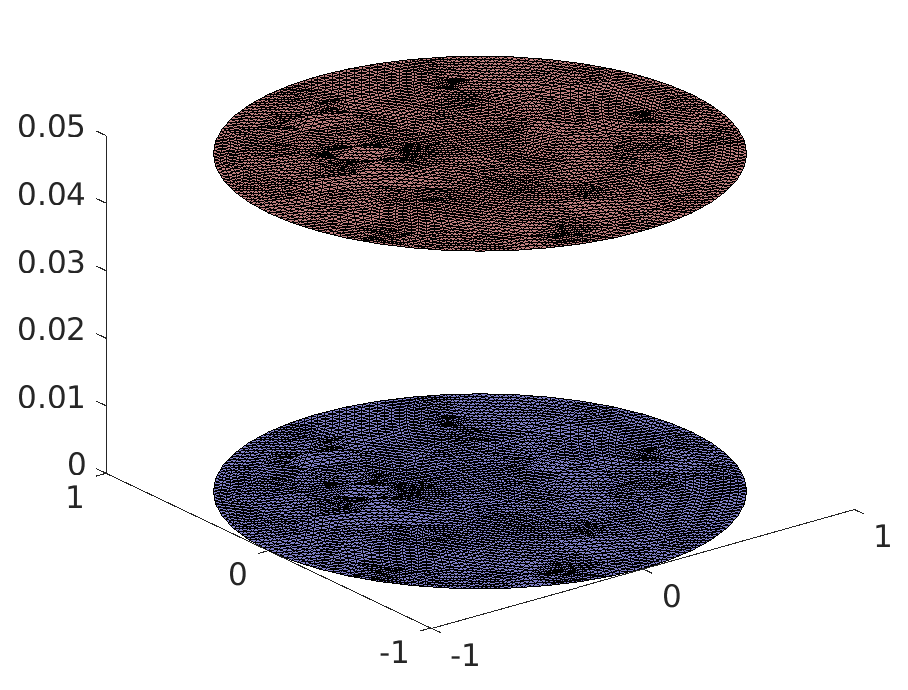
\includegraphics[width=0.48 \textwidth]{fig_article_chap_2/test_case_128/fig_u1u2_hmax0,09_Dt0,001_tt00.eps} 
\quad
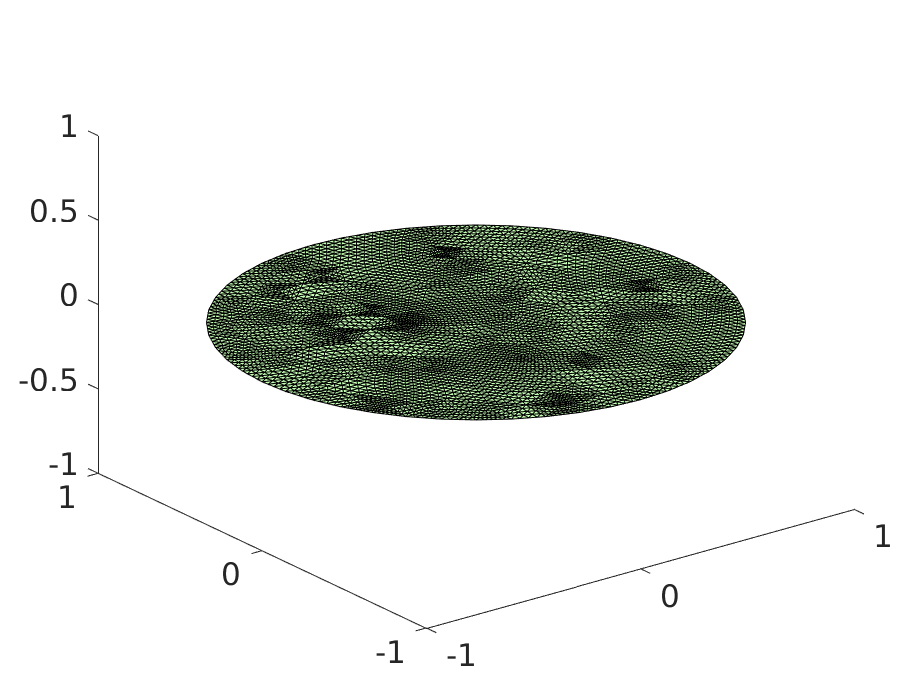
\includegraphics[width=0.48 \textwidth]{fig_article_chap_2/test_case_128/fig_lambda_hmax0,09_Dt0,001_tt02.eps} 
\end{figure}
\onslide<2>
\begin{figure}
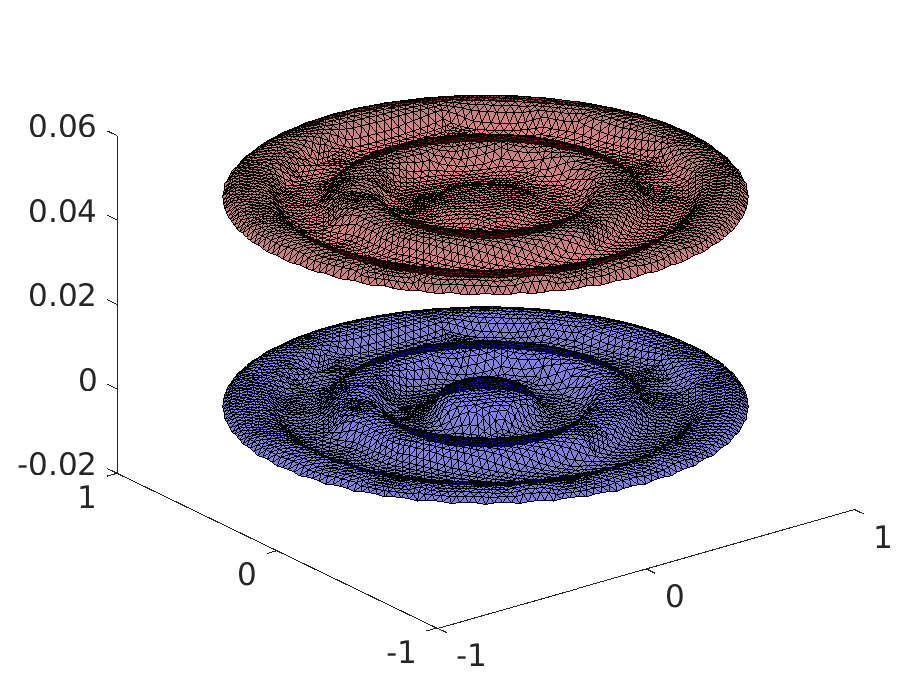
\includegraphics[width=0.48 \textwidth]{fig_article_chap_2/test_case_128/fig_u1u2_hmax0,09_Dt0,001_tt01.eps} 
\quad
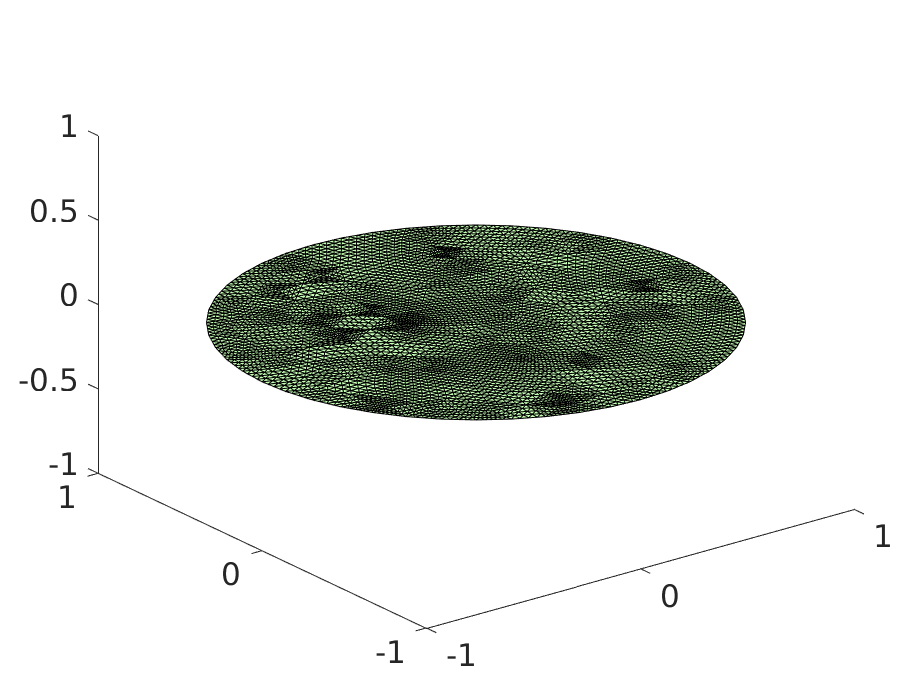
\includegraphics[width=0.48 \textwidth]{fig_article_chap_2/test_case_128/fig_lambda_hmax0,09_Dt0,001_tt02.eps} 
\end{figure}
\onslide<3>
\begin{figure}
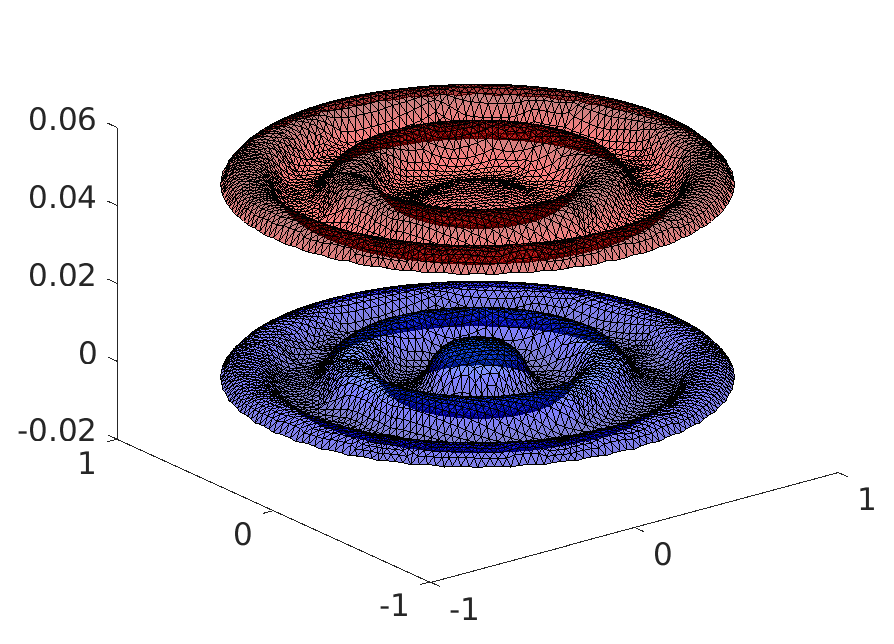
\includegraphics[width=0.48 \textwidth]{fig_article_chap_2/test_case_128/fig_u1u2_hmax0,09_Dt0,001_tt02.eps} 
\quad
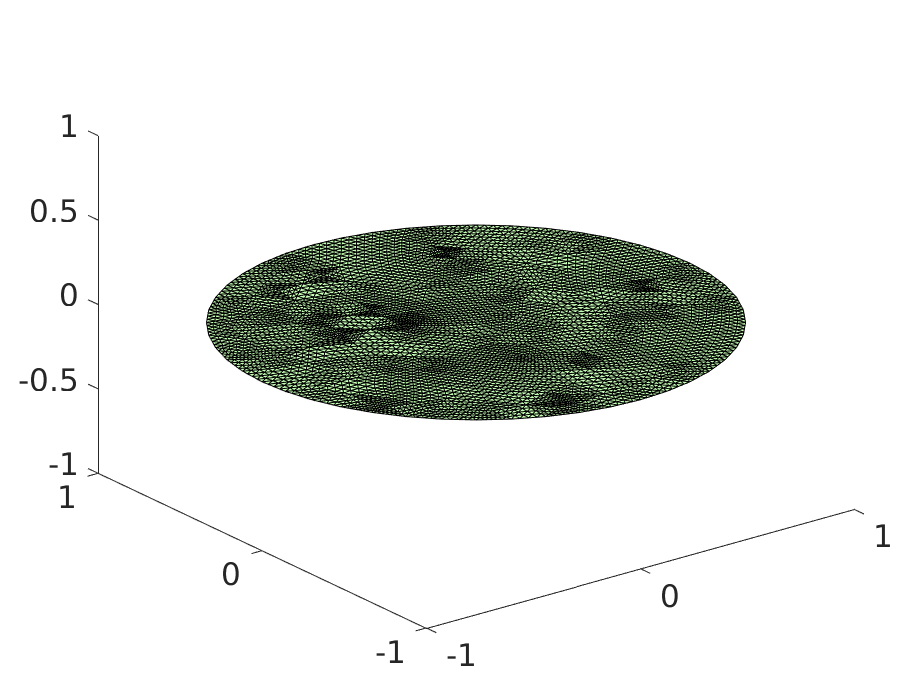
\includegraphics[width=0.48 \textwidth]{fig_article_chap_2/test_case_128/fig_lambda_hmax0,09_Dt0,001_tt02.eps} 
\end{figure}
\onslide<4>
\begin{figure}
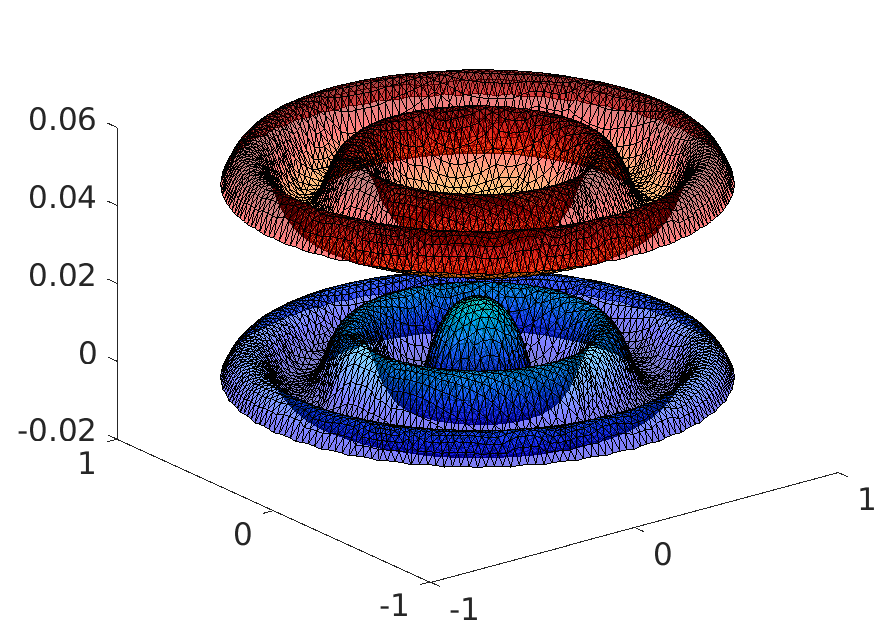
\includegraphics[width=0.48 \textwidth]{fig_article_chap_2/test_case_128/fig_u1u2_hmax0,09_Dt0,001_tt03.eps} 
\quad
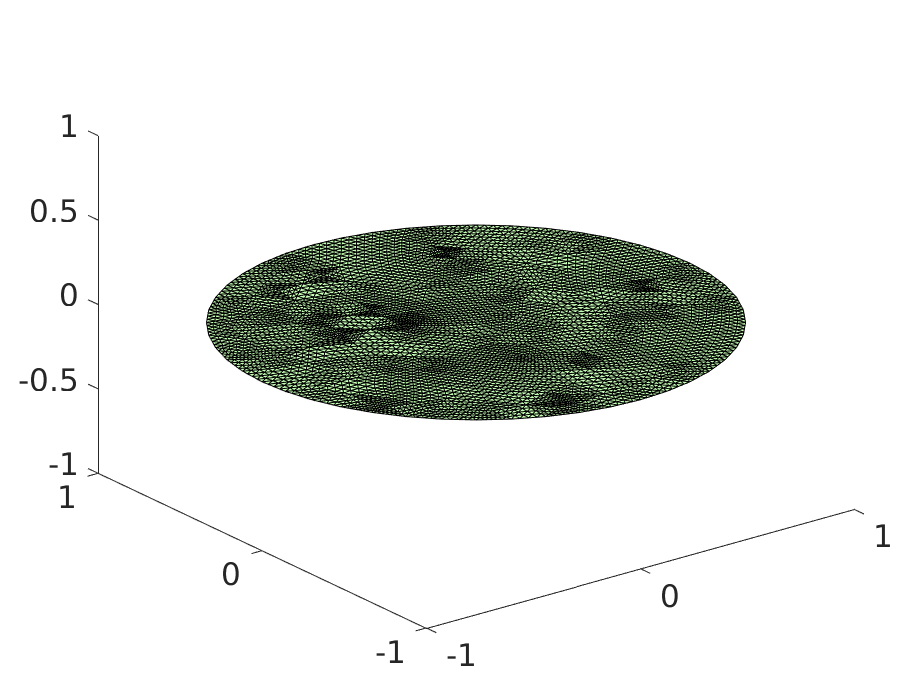
\includegraphics[width=0.48 \textwidth]{fig_article_chap_2/test_case_128/fig_lambda_hmax0,09_Dt0,001_tt02.eps} 
\end{figure}
\onslide<5>
\begin{figure}
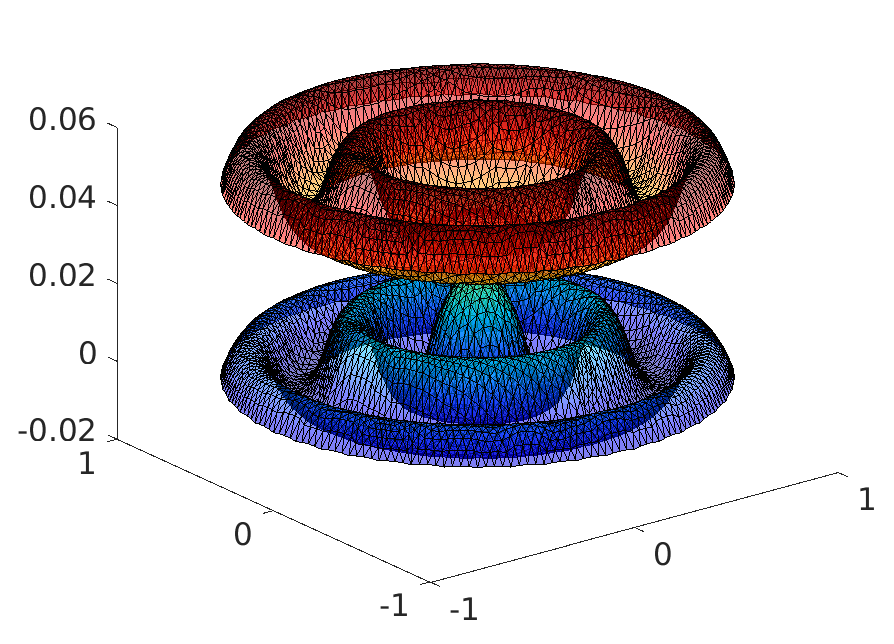
\includegraphics[width=0.48 \textwidth]{fig_article_chap_2/test_case_128/fig_u1u2_hmax0,09_Dt0,001_tt04.eps} 
\quad
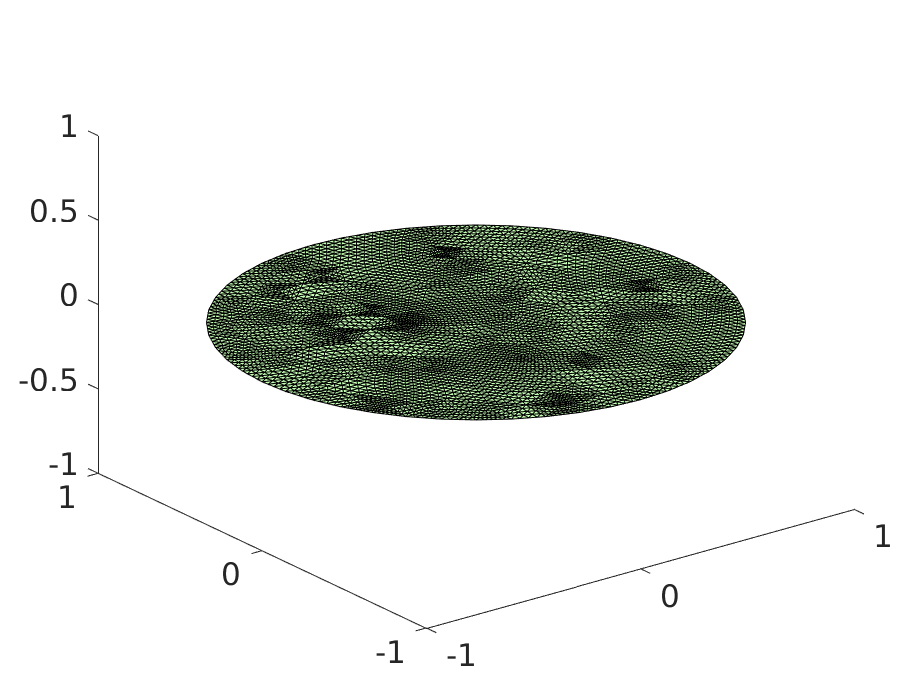
\includegraphics[width=0.48 \textwidth]{fig_article_chap_2/test_case_128/fig_lambda_hmax0,09_Dt0,001_tt02.eps} 
\end{figure}
\onslide<6>
\begin{figure}
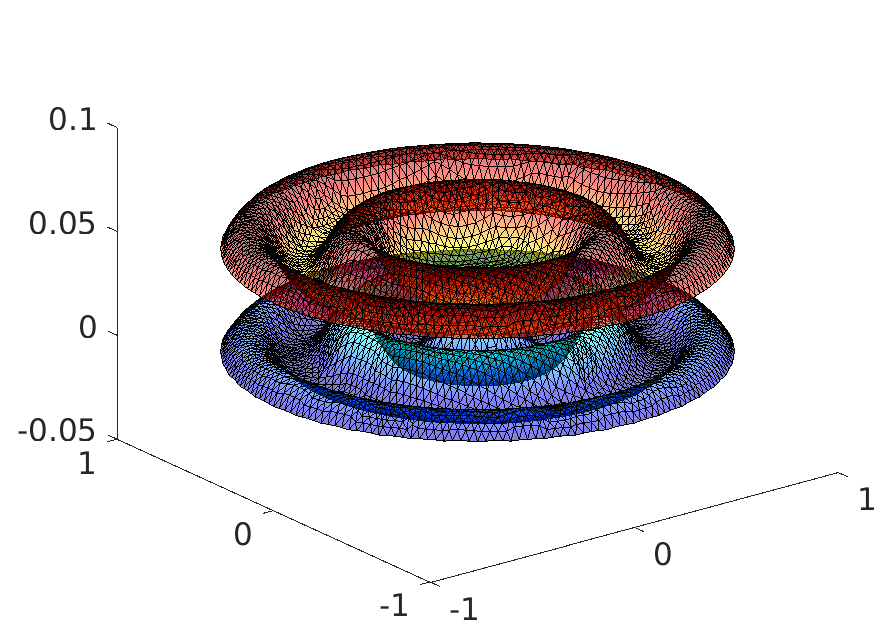
\includegraphics[width=0.48 \textwidth]{fig_article_chap_2/test_case_128/fig_u1u2_hmax0,09_Dt0,001_tt05.eps} 
\quad
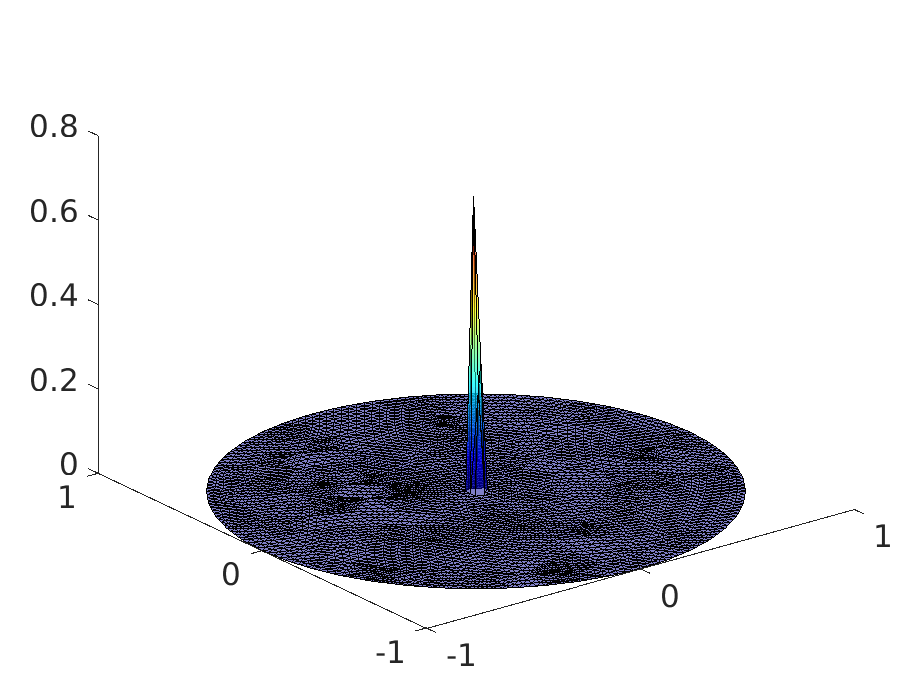
\includegraphics[width=0.48 \textwidth]{fig_article_chap_2/test_case_128/fig_lambda_hmax0,09_Dt0,001_tt05.eps}
\end{figure}
\onslide<7>
\begin{figure}
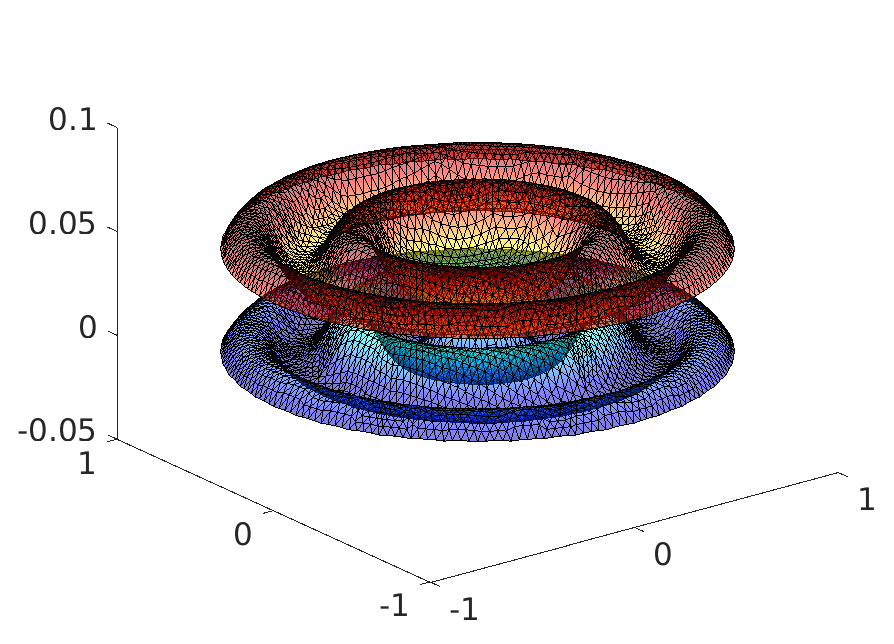
\includegraphics[width=0.48 \textwidth]{fig_article_chap_2/test_case_128/fig_u1u2_hmax0,09_Dt0,001_tt06.eps} 
\quad
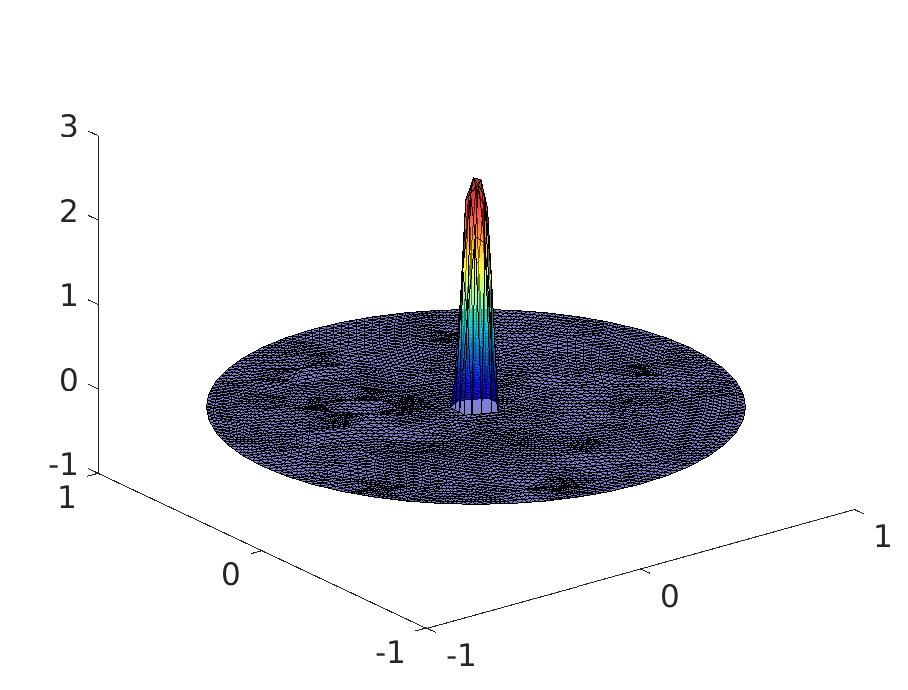
\includegraphics[width=0.48 \textwidth]{fig_article_chap_2/test_case_128/fig_lambda_hmax0,09_Dt0,001_tt06.eps} 
\end{figure}
\onslide<8>
\begin{figure}
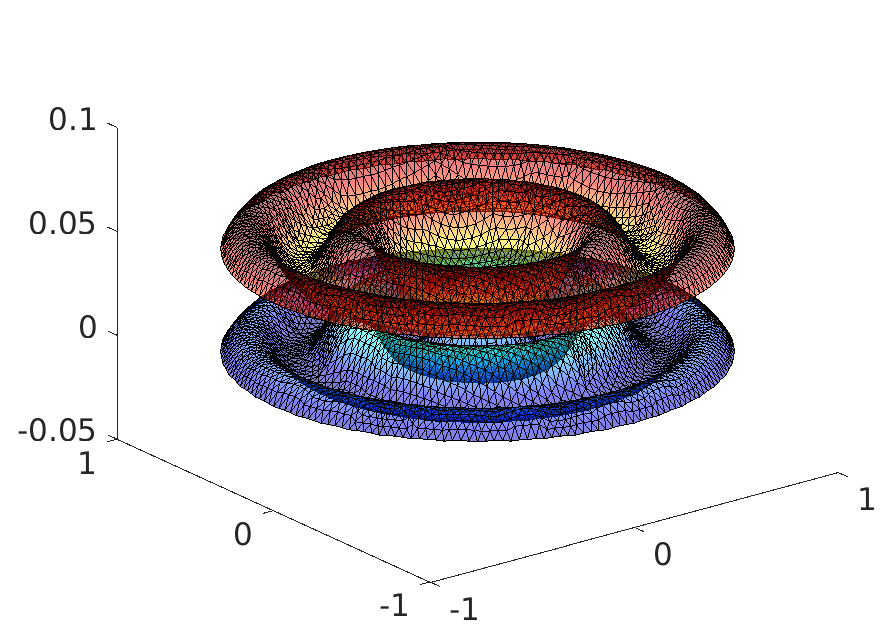
\includegraphics[width=0.48 \textwidth]{fig_article_chap_2/test_case_128/fig_u1u2_hmax0,09_Dt0,001_tt07.eps} 
\quad
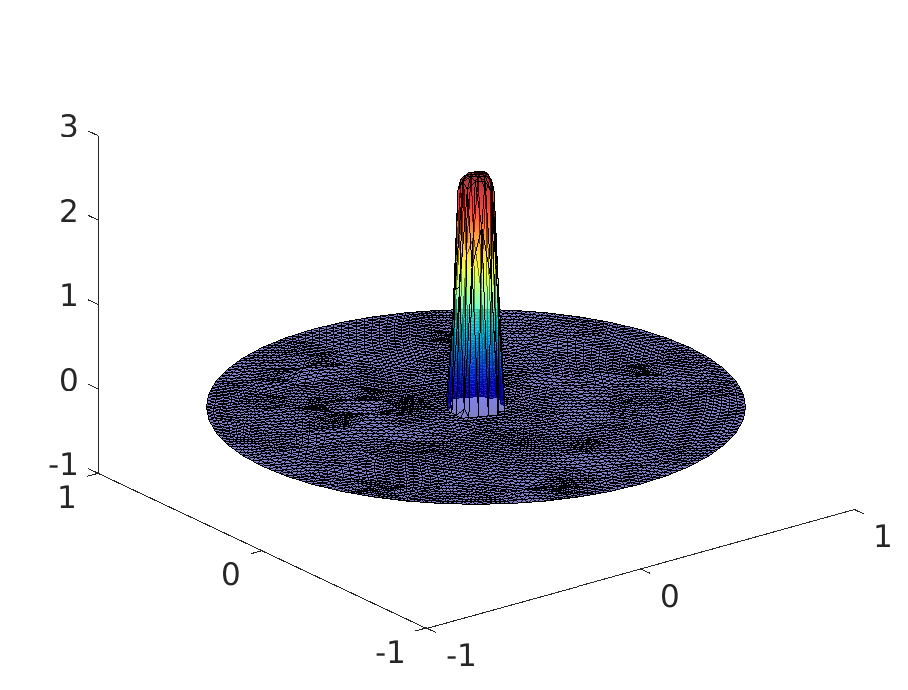
\includegraphics[width=0.48 \textwidth]{fig_article_chap_2/test_case_128/fig_lambda_hmax0,09_Dt0,001_tt07.eps} 
\end{figure}
\onslide<9>
\begin{figure}
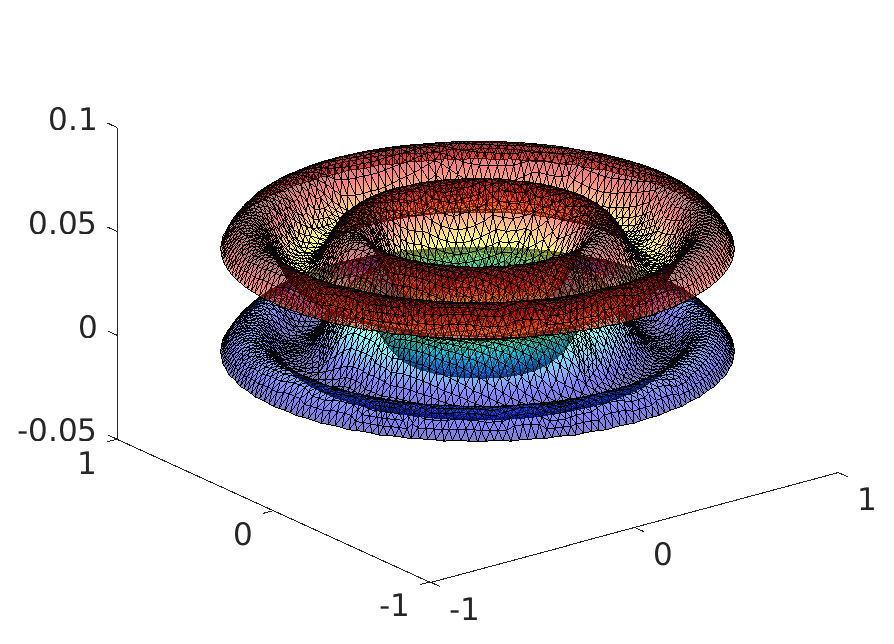
\includegraphics[width=0.48 \textwidth]{fig_article_chap_2/test_case_128/fig_u1u2_hmax0,09_Dt0,001_tt08.eps} 
\quad
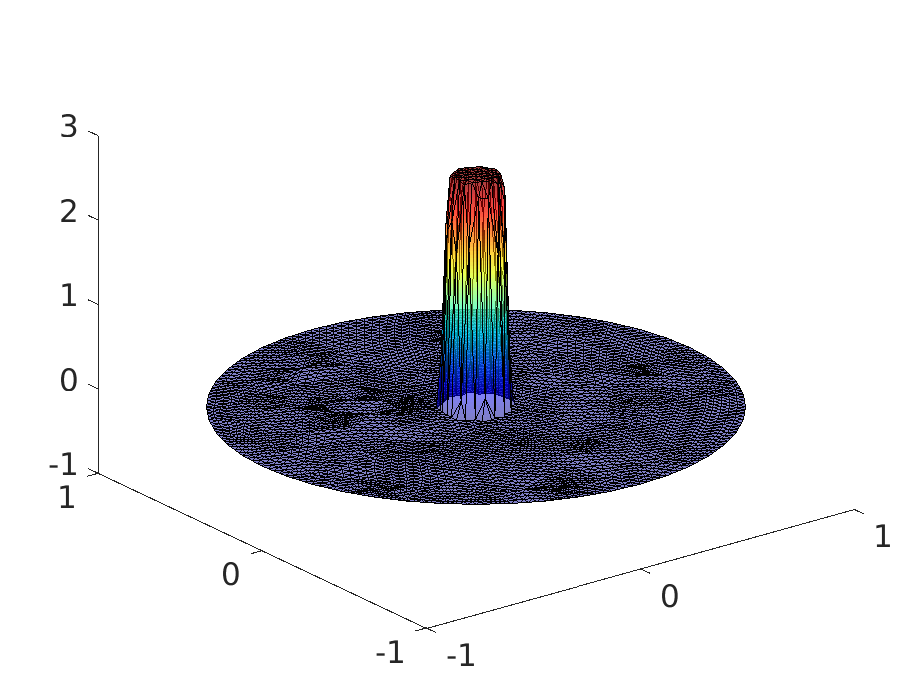
\includegraphics[width=0.48 \textwidth]{fig_article_chap_2/test_case_128/fig_lambda_hmax0,09_Dt0,001_tt08.eps} 
\end{figure}
\onslide<10>
\begin{figure}
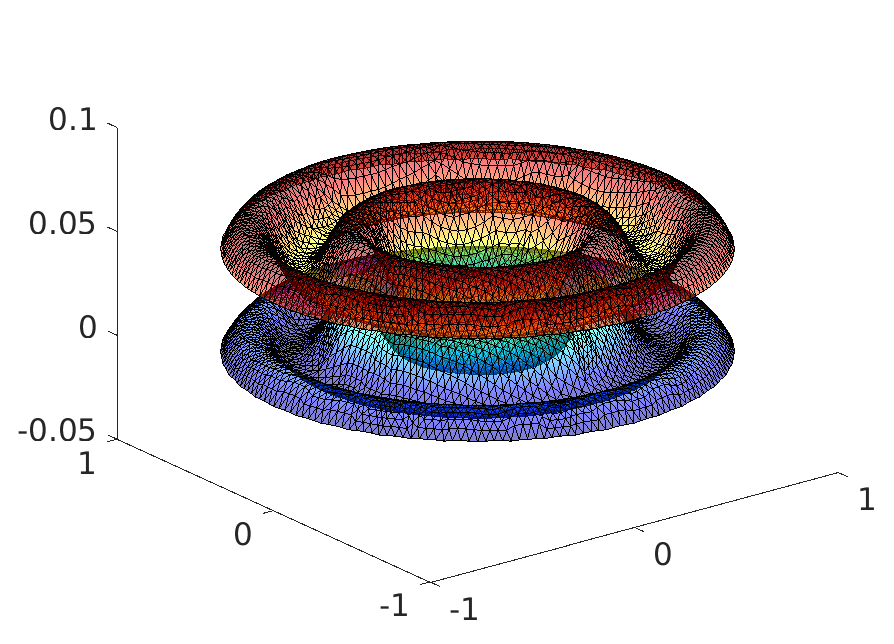
\includegraphics[width=0.48 \textwidth]{fig_article_chap_2/test_case_128/fig_u1u2_hmax0,09_Dt0,001_tt09.eps} 
\quad
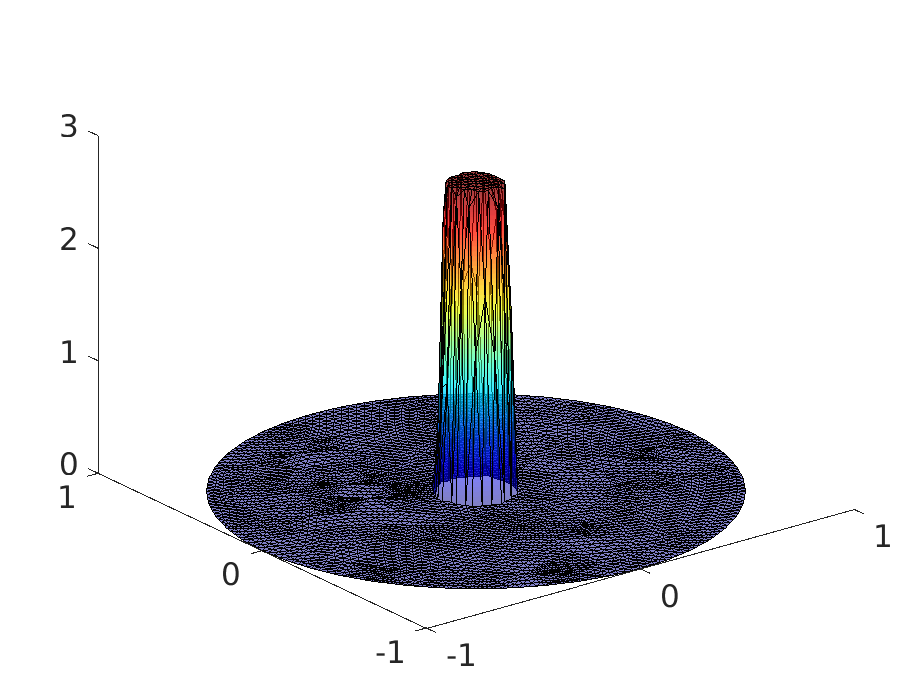
\includegraphics[width=0.48 \textwidth]{fig_article_chap_2/test_case_128/fig_lambda_hmax0,09_Dt0,001_tt09.eps} 
\end{figure}
\onslide<11>
\begin{figure}
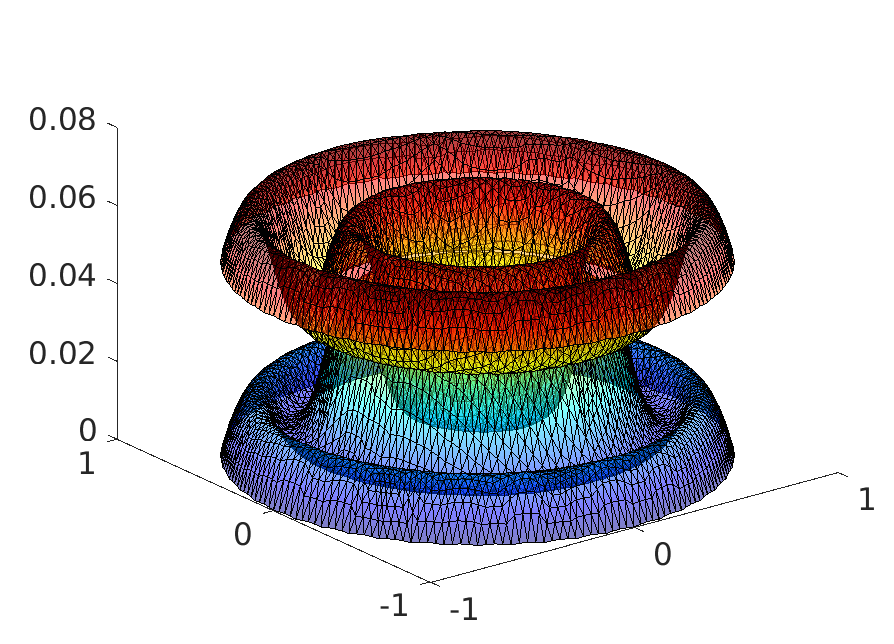
\includegraphics[width=0.48 \textwidth]{fig_article_chap_2/test_case_128/fig_u1u2_hmax0,09_Dt0,001_tt10.eps} 
\quad
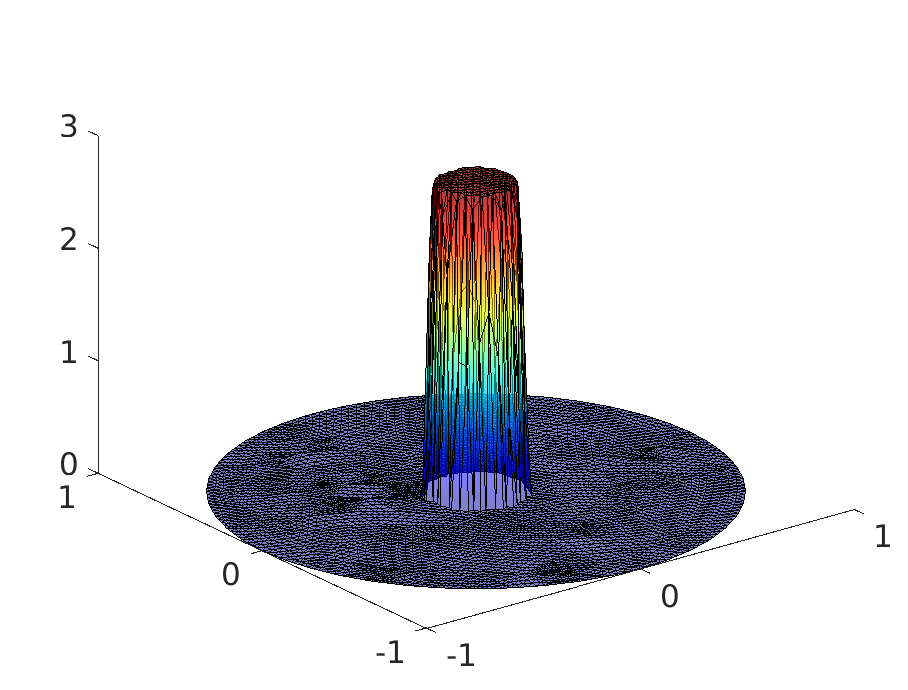
\includegraphics[width=0.48 \textwidth]{fig_article_chap_2/test_case_128/fig_lambda_hmax0,09_Dt0,001_tt10.eps} 
\end{figure}
\onslide<12>
\begin{figure}
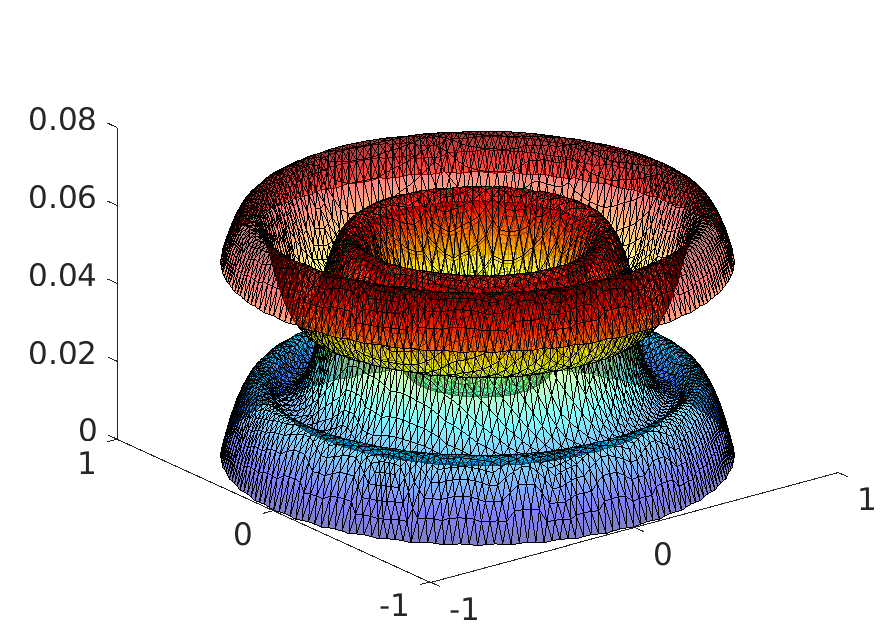
\includegraphics[width=0.48 \textwidth]{fig_article_chap_2/test_case_128/fig_u1u2_hmax0,09_Dt0,001_tt11.eps} 
\quad
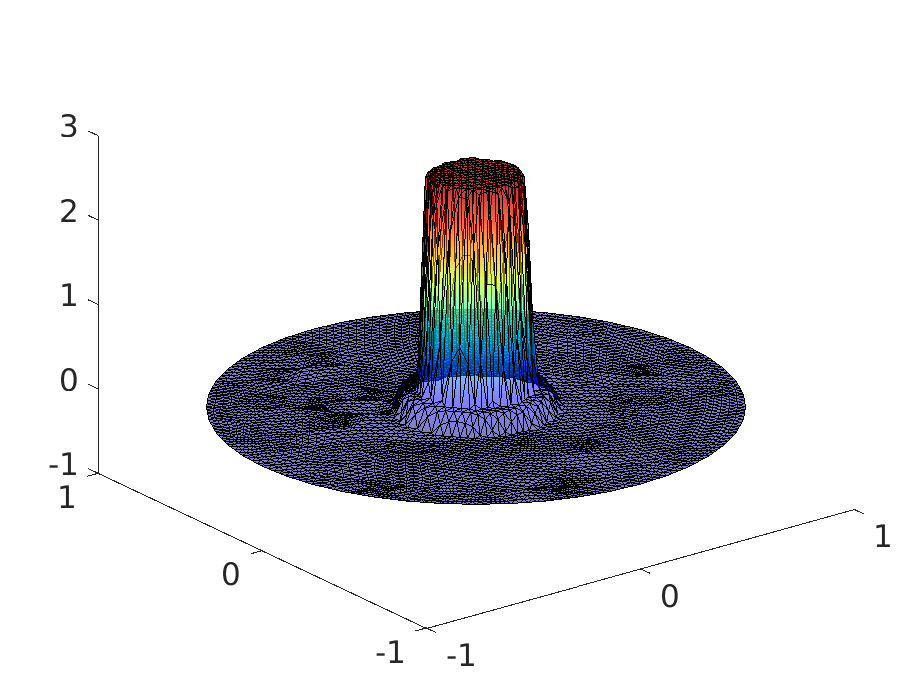
\includegraphics[width=0.48 \textwidth]{fig_article_chap_2/test_case_128/fig_lambda_hmax0,09_Dt0,001_tt11.eps} 
\end{figure}
\onslide<13>
\vspace*{-0.3 cm}
\begin{figure}
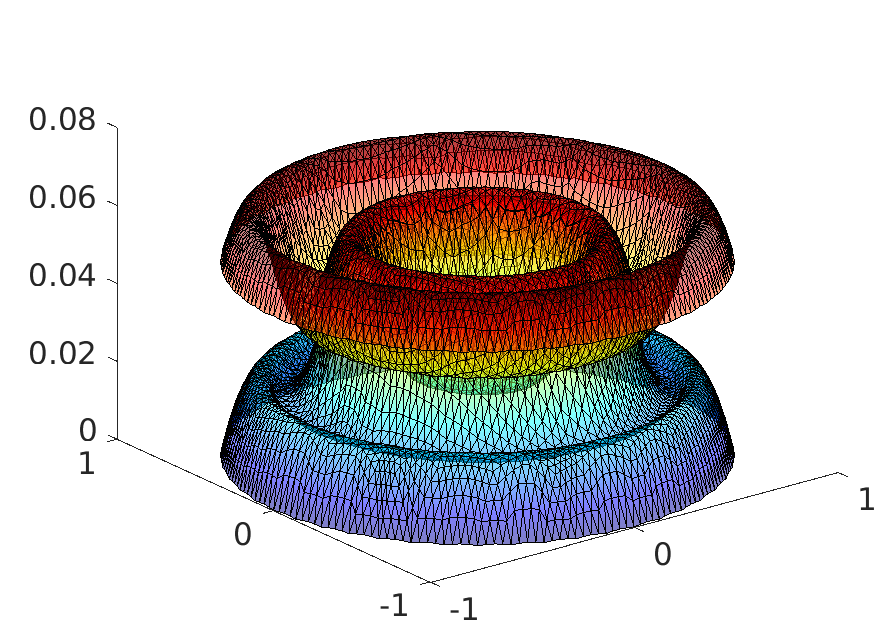
\includegraphics[width=0.48 \textwidth]{fig_article_chap_2/test_case_128/fig_u1u2_hmax0,09_Dt0,001_tt12.eps} 
\quad
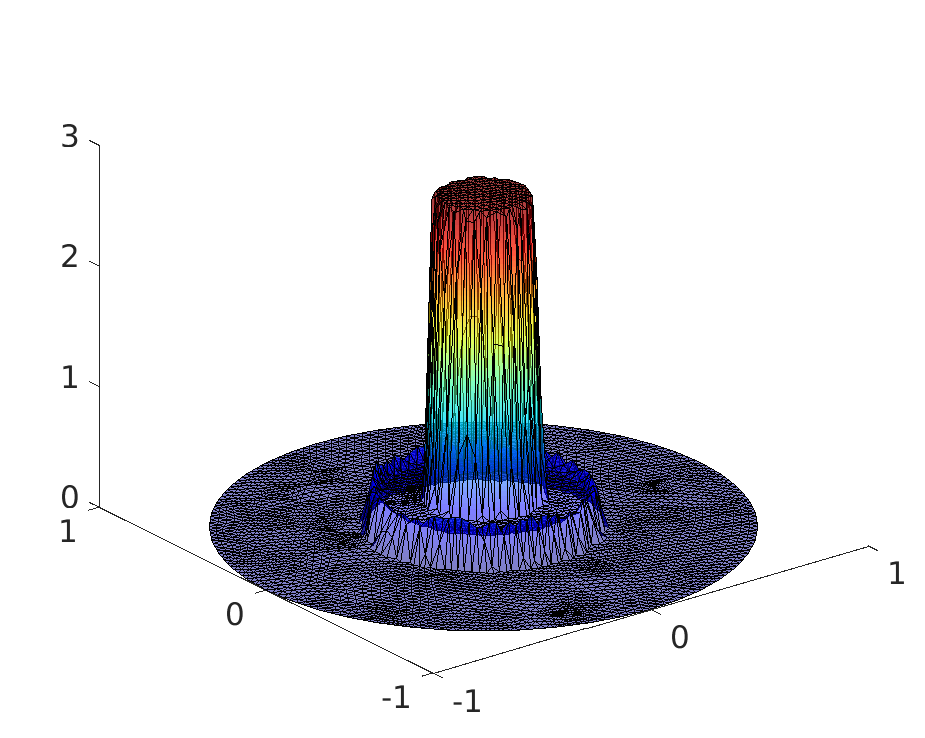
\includegraphics[width=0.48 \textwidth]{fig_article_chap_2/test_case_128/fig_lambda_hmax0,09_Dt0,001_tt12.eps} 
\end{figure}
\onslide<14>
\begin{figure}
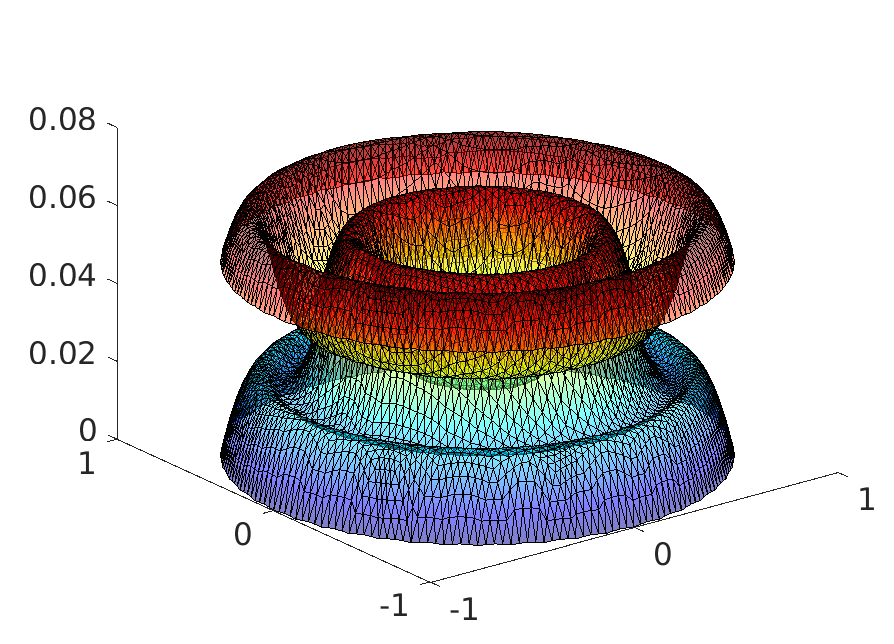
\includegraphics[width=0.48 \textwidth]{fig_article_chap_2/test_case_128/fig_u1u2_hmax0,09_Dt0,001_tt14.eps} 
\quad
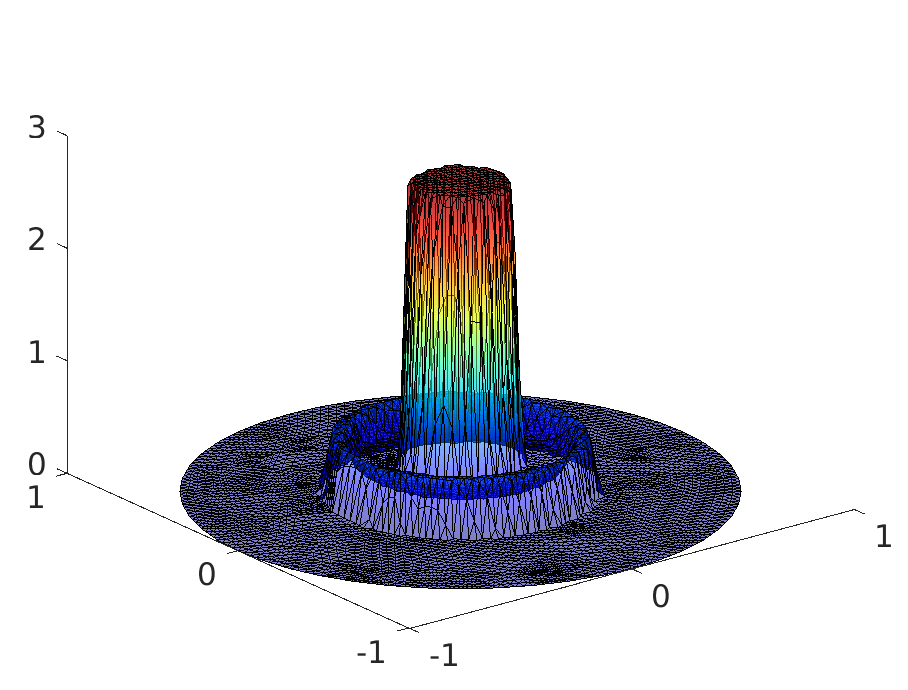
\includegraphics[width=0.48 \textwidth]{fig_article_chap_2/test_case_128/fig_lambda_hmax0,09_Dt0,001_tt14.eps} 
\end{figure}
\end{overprint}
\end{frame}

%%% NM ADAPTIVITY
% \begin{frame}
% \frametitle{Newton-min adaptivity}
% \begin{figure}
% \centering
% 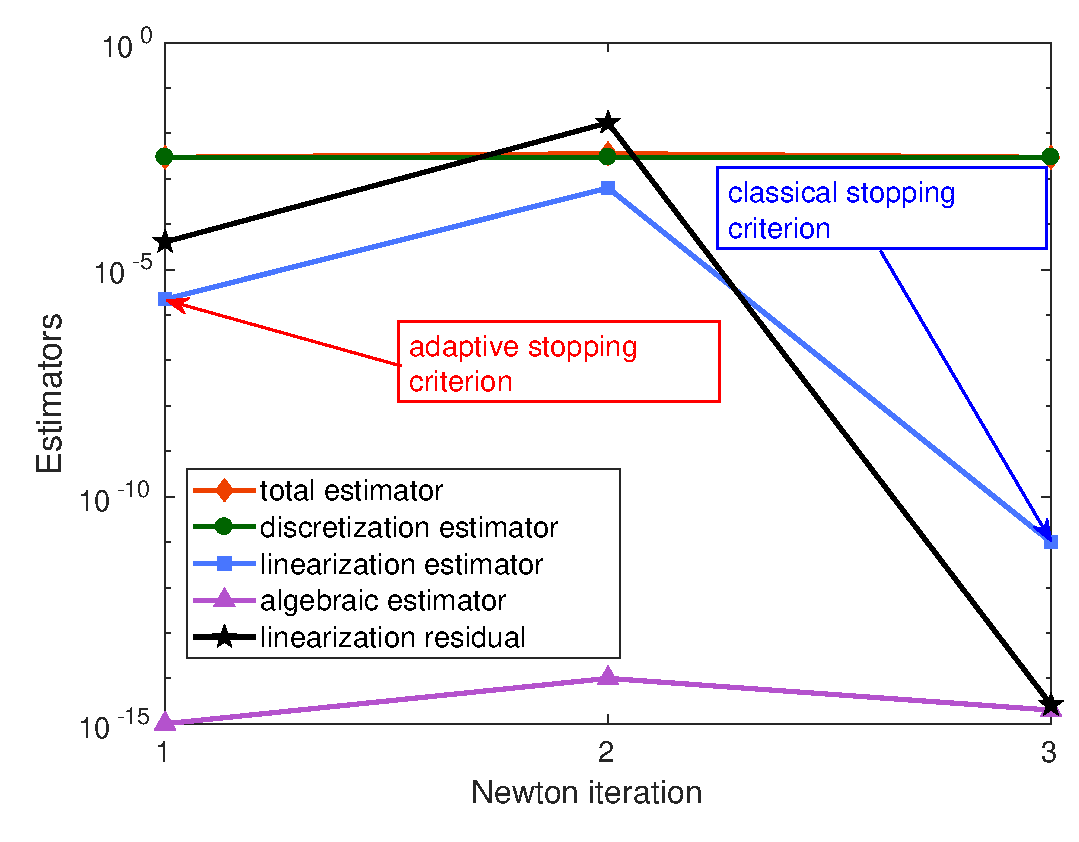
\includegraphics[width = 0.47 \textwidth]{fig_article_chap_2/test_case_128/test_case_NM_time84_newton_estimator} \quad
% 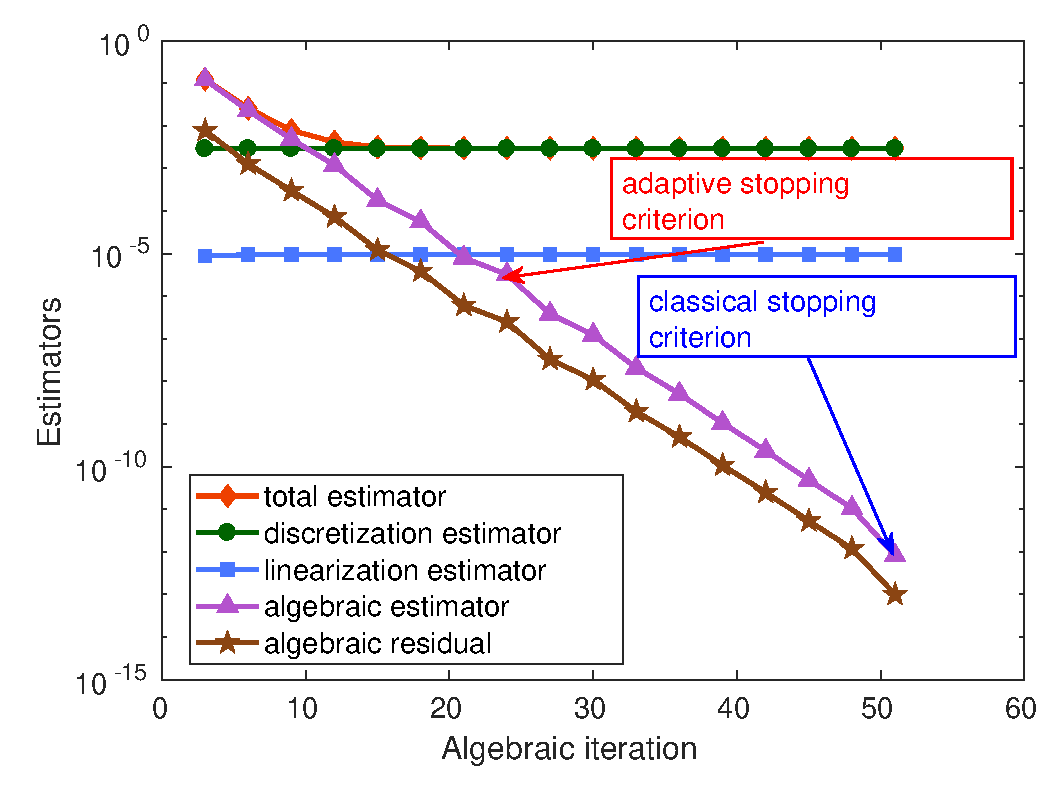
\includegraphics[width = 0.49 \textwidth]{fig_article_chap_2/test_case_128/test_case_NM_time84_gmres_estimator_1stNewton}
% \end{figure}
% \end{frame}
%
\begin{frame}
\frametitle{Newton--Fischer--Burmeister adaptivity}
\textcolor{red}{\bm{$\gammalin=\gammaalg=10^{-3}$}}
\begin{figure}
\centering
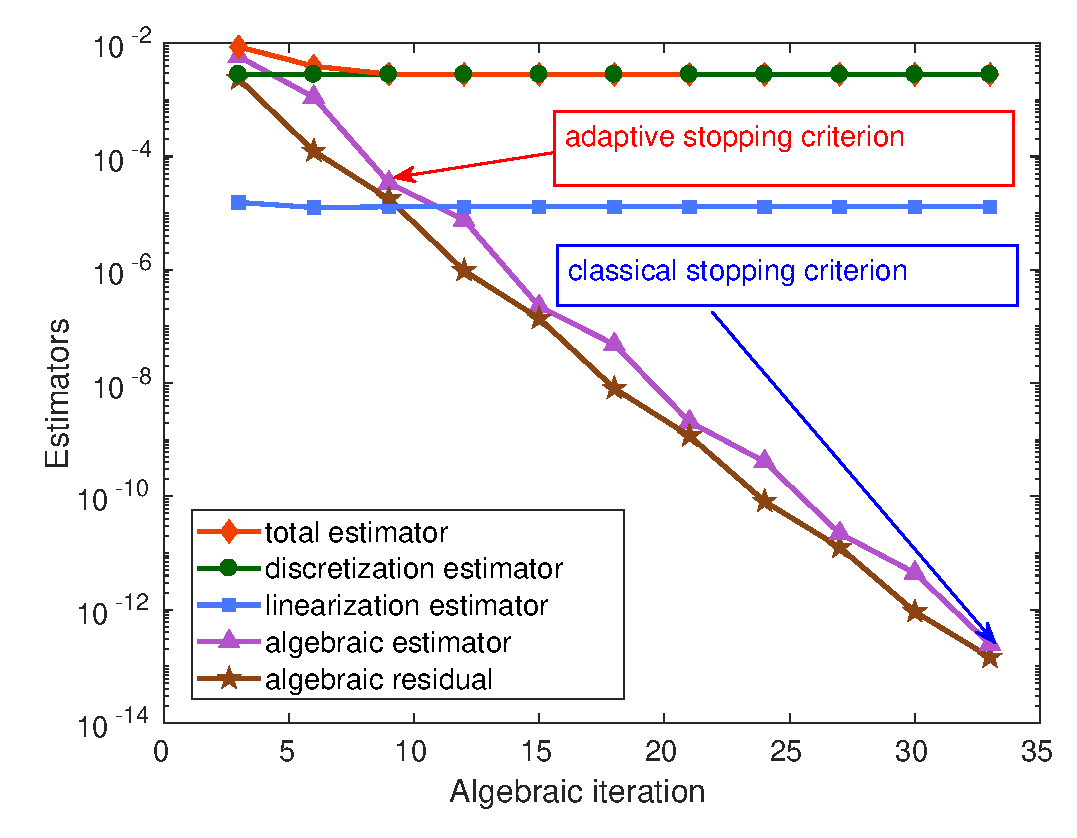
\includegraphics[scale=0.44]{fig_article_chap_2/test_case_1_iter_11_estimator_gmres_1st_newton_iter}
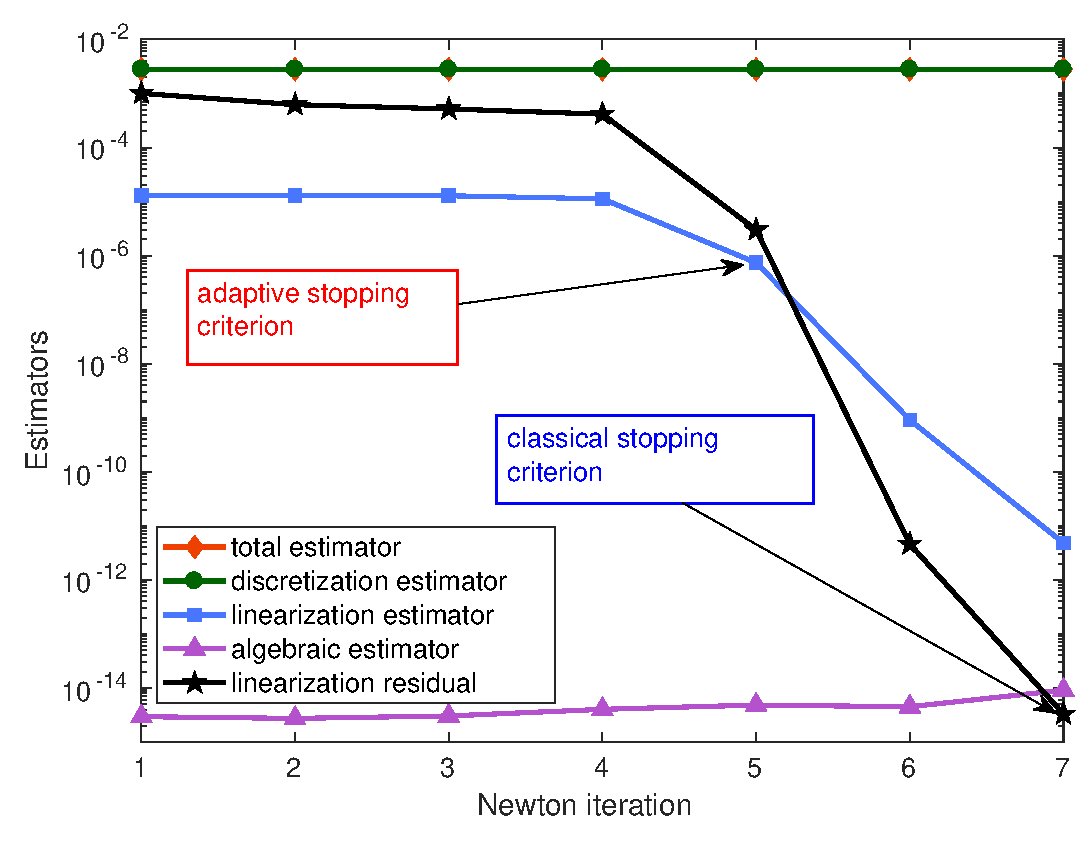
\includegraphics[scale=0.44]{fig_article_chap_2/test_case_1_iter_11_estimator_newton_iter}
\end{figure}
\end{frame}
%
%% NM PERFORMANCE
% \begin{frame}
% \frametitle{Newton--min performance}
% \begin{figure}
% \centering
% \includegraphics[width = 0.47 \textwidth]{fig_article_chap_2/test_case_128/number_newton_min_iter_time_gamma_lin_alg_10-3} \quad
% 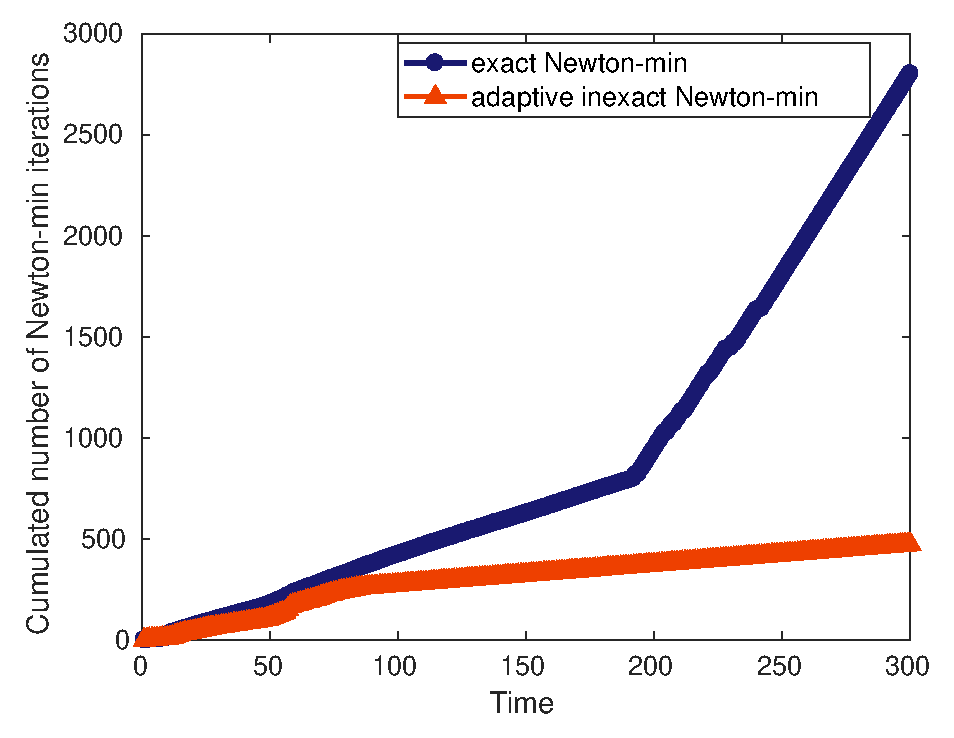
\includegraphics[width = 0.49 \textwidth]{fig_article_chap_2/test_case_128/cumulated_number_newton_min_iter_time_gamma_lin_alg_10-3}
% \end{figure}
% \end{frame}
%
\begin{frame}
\frametitle{Newton--Fischer--Burmeister performance}
\begin{figure}
\centering
% \includegraphics[width=0.48 \textwidth]{fig_article_chap_2/test_case_128/Number_Newton_FB_iter_time_gamma_10-3} 
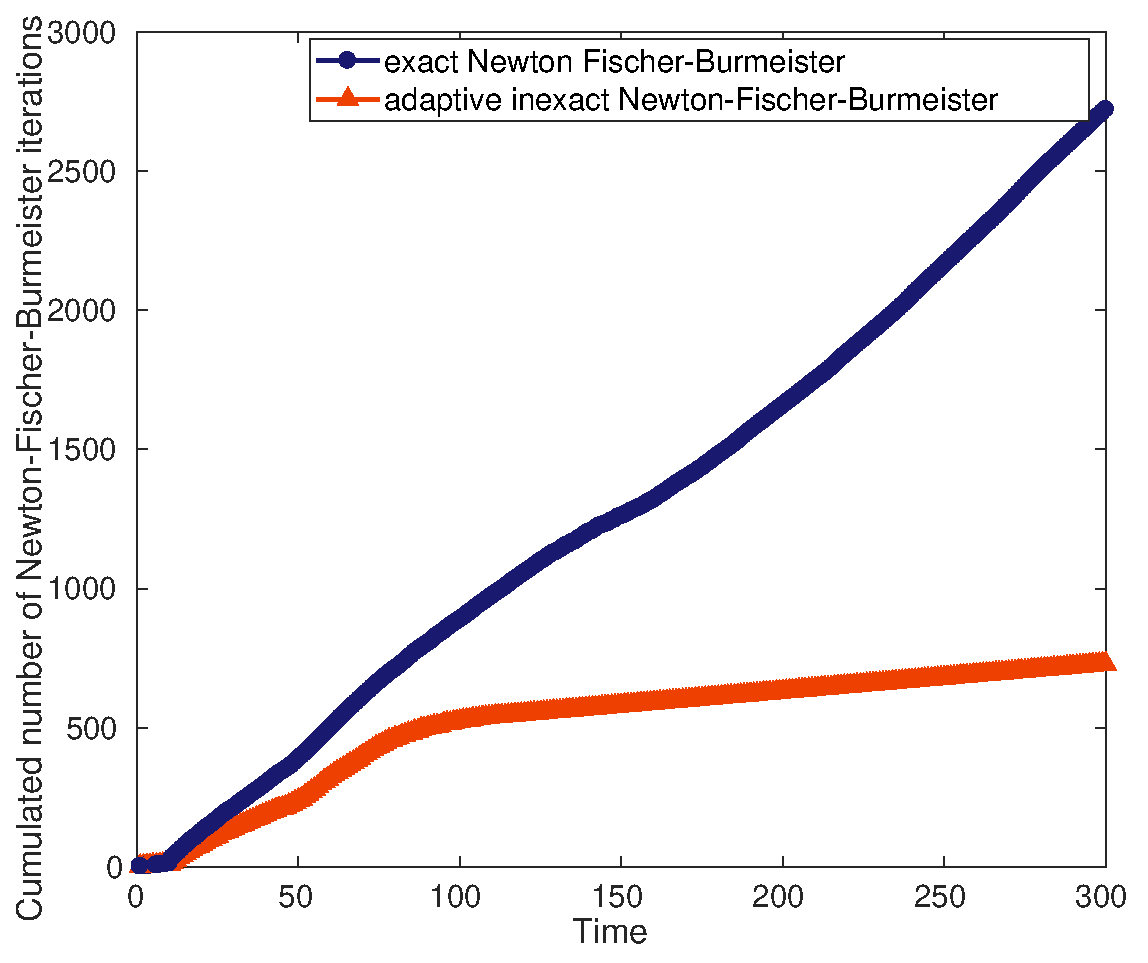
\includegraphics[width=0.48 \textwidth]{fig_article_chap_2/test_case_128/Cumulated_number_Newton_FB_iter_time_gamma_10-3}
\quad
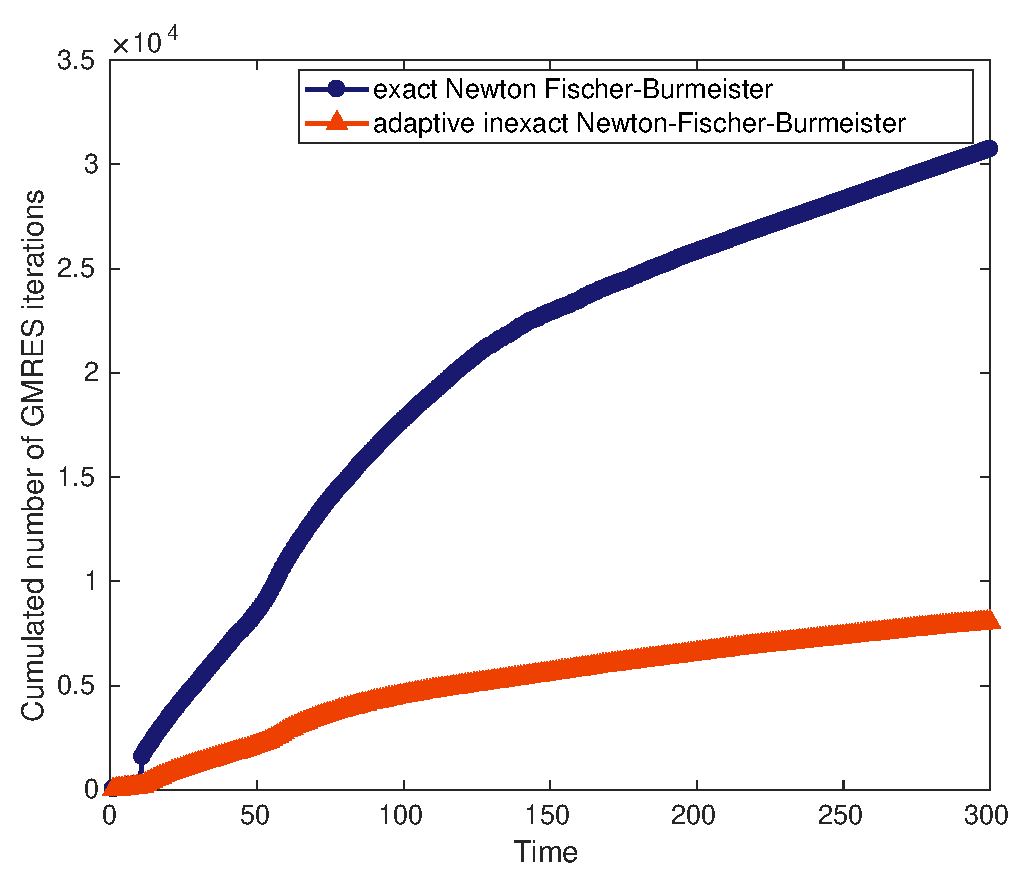
\includegraphics[width=0.48 \textwidth]{fig_article_chap_2/test_case_128/cumulated_number_gmresFB_iter_time_gamma_lin_alg_10-3}
\end{figure}
\end{frame}
%
% \begin{frame}
% \frametitle{GMRES overall performance}
% \begin{figure}
% \centering
% 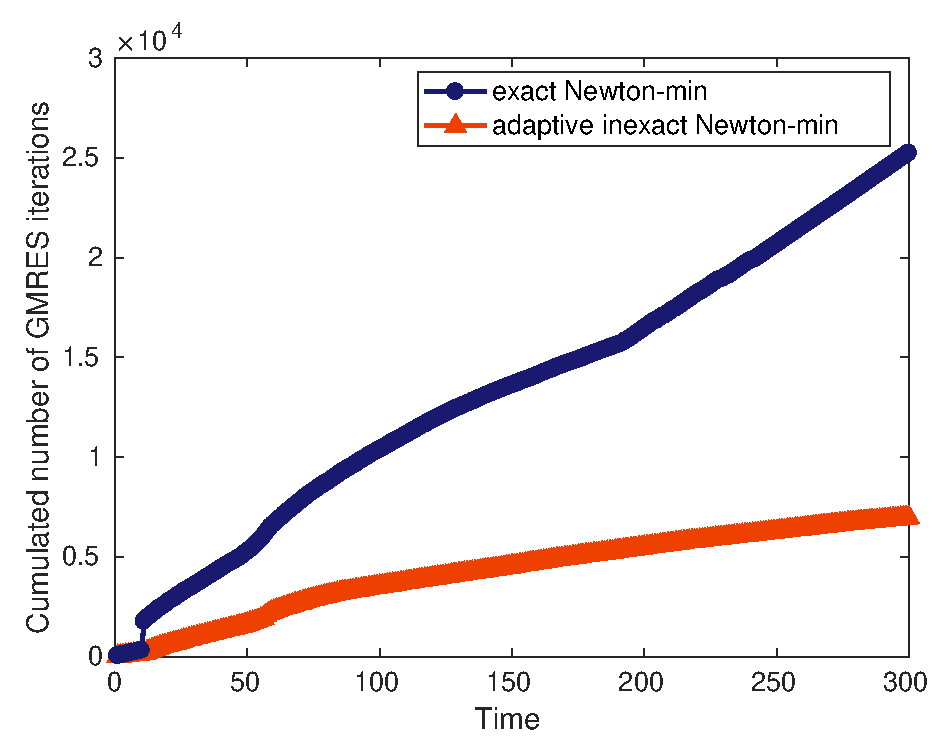
\includegraphics[width = 0.48 \textwidth]{fig_article_chap_2/test_case_128/cumulated_number_gmresNM_iter_time_gamma_lin_alg_10-3}
% \quad
% 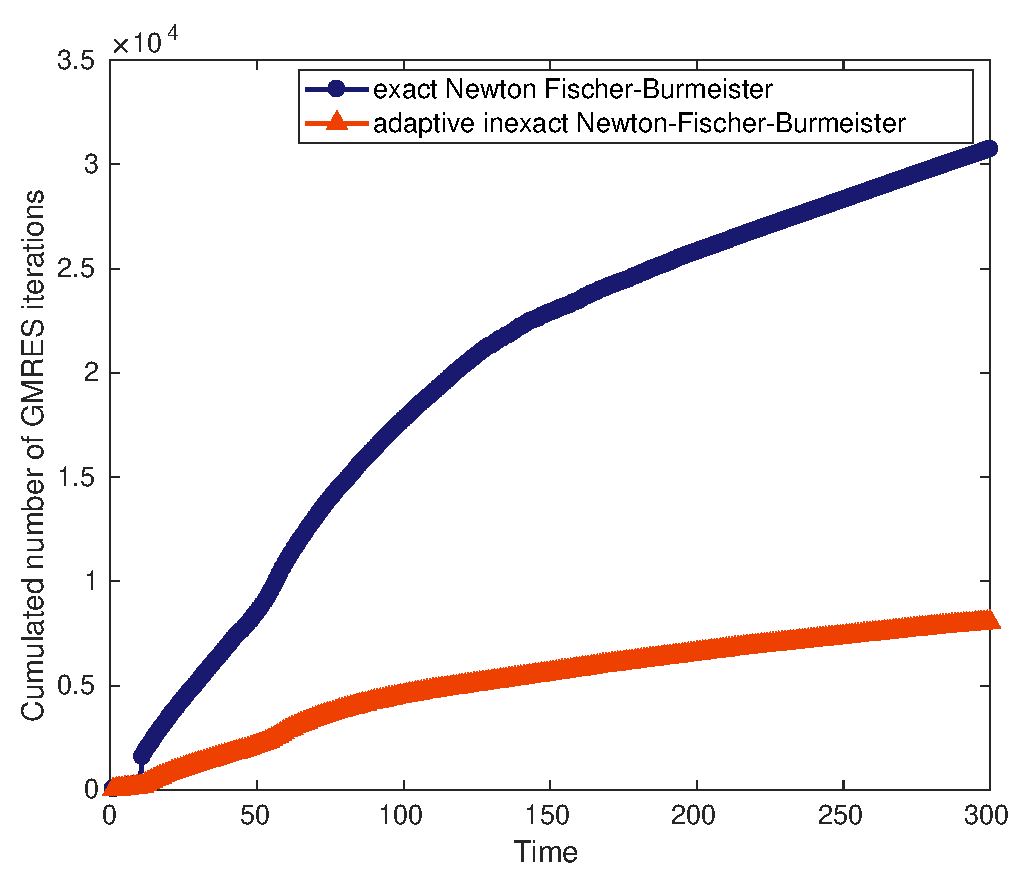
\includegraphics[width=0.48 \textwidth]{fig_article_chap_2/test_case_128/cumulated_number_gmresFB_iter_time_gamma_lin_alg_10-3}
% \end{figure}
% \end{frame}
%
%% ADAPTIVE NM ACCURACY
% \begin{frame}
% \frametitle{Adaptive inexact Newton accuracy}
% \textcolor{cadmiumgreen}{\textbf{Newton-min}}
% \invisible<1>{
% \begin{table}
% \centering
% \begin{tabular}{|l|l|l|l|l|l|}
% \hline
% $\gammaalg=\gammalin=10^{-3}$                                                         & $n=1$ & $n=11$ & $n=70$ & $n=150$ & $n=300$ \\
%  \hline
% $\left\|u_{1h}^{\mathrm{exact}} - u_{1h}^{\mathrm{adapt}}\right\|_{\Omega}$           &     $ 3.7 \times 10^{-7}$  &   $9.7 \times 10^{-7}$    &   $6.3 \times 10^{-7}$     &   $3.3 \times 10^{-6}$       &    $6.3 \times 10^{-6}$     \\ \hline
% $\left\|u_{2h}^{\mathrm{exact}} - u_{2h}^{\mathrm{adapt}}\right\|_{\Omega}$           &   $2.4 \times 10^{-7}$    &    $5.5 \times 10^{-7}$    &    $5.8 \times 10^{-7}$    &  $2.7 \times 10^{-6}$       &   $6.3 \times 10^{-6}$      \\ \hline
% $\left\|\lambda_{h}^{\mathrm{exact}} - \lambda_{h}^{\mathrm{adapt}}\right\|_{\Omega}$ &   $0$    &   $1.9 \times 10^{-4}$     &     $1.9 \times 10^{-4}$   &    $2.5 \times 10^{-4}$     &    $4.9 \times 10^{-8}$     \\ \hline
% \end{tabular}
% \end{table}
% \invisible<2>{
% \textcolor{cadmiumgreen}{\textbf{Newton--Fischer--Burmeister}}
% \invisible<3>{
% \begin{table}[]
% \begin{tabular}{|c|c|c|c|c|c|}
% \hline
% $\gammaalg=\gammalin=10^{-3}$                                                         & $n=1$                    & $n=11$                   & $n=70$                   & $n=150$                  & $n=300$                  \\ \hline
% $\left\|u_{1h}^{\mathrm{exact}} - u_{1h}^{\mathrm{adapt}}\right\|_{\Omega}$           & $4.8 \times 10^{-7}$ & $3.2 \times 10^{-6}$ & $8.9 \times 10^{-7}$ & $9.1 \times 10^{-6}$ & $2.5 \times 10^{-5}$ \\ \hline
% $\left\|u_{2h}^{\mathrm{exact}} - u_{2h}^{\mathrm{adapt}}\right\|_{\Omega}$           & $3.3 \times 10^{-7}$ & $3.3 \times 10^{-6}$ & $9.6 \times 10^{-7}$ & $6.3 \times 10^{-6}$ & $2.5 \times 10^{-5}$ \\ \hline
% $\left\|\lambda_{h}^{\mathrm{exact}} - \lambda_{h}^{\mathrm{adapt}}\right\|_{\Omega}$ & 0                        & $7.95 \times 10^{-3}$ & $3.2 \times 10^{-4}$ & $2.2 \times 10^{-2}$ & $2.2 \times 10^{-7}$ \\ \hline
% \end{tabular}
% \end{table}
% \invisible<4>{
% }}}}
% \end{frame}
%
